% Type of the document
\documentclass{beamer}

% elementary packages:
\usepackage{graphicx}
\usepackage[latin1]{inputenc}
\usepackage[T1]{fontenc}
\usepackage[english]{babel}
\usepackage{listings}
\usepackage{xcolor}
\usepackage{eso-pic}
\usepackage{mathrsfs}
\usepackage{url}
\usepackage{amssymb}
\usepackage{amsmath}
\usepackage{multirow}
\usepackage{hyperref}
\usepackage{booktabs}
\usepackage{tikz}

% additional packages
\usepackage{bbm}

% packages supplied with ise-beamer:
\usepackage{cooltooltips}
\usepackage{colordef}
\usepackage{beamerdefs}
\usepackage{lvblisting}

% Change the pictures here:
% logobig and logosmall are the internal names for the pictures: do not modify them. 
% Pictures must be supplied as JPEG, PNG or, to be preferred, PDF
\pgfdeclareimage[height=2cm]{logobig}{hulogo}
% Supply the correct logo for your class and change the file name to "logo". The logo will appear in the lower
% right corner:
\pgfdeclareimage[height=0.7cm]{logosmall}{Figures/LOB_Logo}

% Title page outline:
% use this number to modify the scaling of the headline on title page
\renewcommand{\titlescale}{1.0}
% the title page has two columns, the following two values determine the percentage each one should get
\renewcommand{\titlescale}{1.0}
\renewcommand{\leftcol}{0.6}

% Define the title.Don't forget to insert an abbreviation instead 
% of "title for footer". It will appear in the lower left corner:
\title[QML estimation of an ARCH(1) model]{Monte Carlo Simulation of a QML estimation of an ARCH(1) model}
% Define the authors:
\authora{Paulina Kurowska} % a-c
\authorb{Bingling Wang}
\authorc{}

% Define any internet addresses, if you want to display them on the title page:
\def\linka{http://lvb.wiwi.hu-berlin.de}%link to github doesnt work!!!
\def\linkb{}
\def\linkc{}
% Define the institute:
\institute{Ladislaus von Bortkiewicz Chair of Statistics \\
Humboldt--Universitaet zu Berlin \\}

% Comment the following command, if you don't want, that the pdf file starts in full screen mode:
\hypersetup{pdfpagemode=FullScreen}


%Start of the document
\begin{document}

% create the title slide, layout controlled in beamerdefs.sty and the foregoing specifications
\frame[plain]{
\titlepage
}

% The titles of the different sections of you talk, can be included via the \section command. The title will be displayed in the upper left corner. To indicate a new section, repeat the \section command with, of course, another section title
%%%%%%%%%%%%%%%%%%%%%%%%%%%%%%%%%%%%%%%%%%%%%%%%%%%%%%%%%%%%%%%%%%%%%%%%%%%%%%%%%%%%%%%%%%%%%%%%%%%%%%%%%%%%%%%%%%%%%%%%
\section{Introduction}

\section{outline}
	\useheadtemplate{%
		\raisebox{-0.75cm}{\parbox{\textwidth}{%
				\footnotesize{\color{isegray}%
					\insertsection\ \leavevmode\leaders\hrule height3.2pt depth-2.8pt\hfill\kern0pt\ }}}
	}
	
	\frame{
		\frametitle{Outline}
		
		\begin{enumerate}
			\item ARCH(1) model
			\item Maximum Likelihood estimation
			\item Requirements
			\item Monte Carlo Simulation
			\item simulation Results
			\item Applications
		\end{enumerate}
	}

% No number on outline slide
\useheadtemplate{%
    \raisebox{-0.75cm}{\parbox{\textwidth}{%
            \footnotesize{\color{isegray}%
                \insertsection\ \leavevmode\leaders\hrule height3.2pt depth-2.8pt\hfill\kern0pt\ \thesection-\thepage}}}}
\setcounter{section}{1}

	\section{ARCH(1) Model}
	
	%%%%%%%%%%%%%%%%%%%%%%%%%%%%%%%%%%%%%%%%%%%%%%%%%%%%%%%%%%%%%%%%%%%%%%%%%%%%%%%%%%%%%%%%%%%%%%%%%%%%%%%%%%%%%%%%%%%%%%%%
	\subsection{General ideas}

\frame[containsverbatim]{
		\frametitle{Properties of ARCH(1) process}
		
		\begin{itemize}
			\item Necessary and sufficient condition for weak stationarity of a semi strong ARCH(1) process is\(\alpha<1\)
			\item 
		\end{itemize}
	}
\frame[containsverbatim]{
		\frametitle{Quasi Maximum likelihood Estimation (QMLE)}
		\begin{itemize}
			\item If \(Z_{t}\) is not normally distributed, \(\hat{\theta}\) is consistent, but not efficient.
			In this case the method is interpreted as quasi ML (QML). 
			\item 
		\end{itemize}
	}

%%%%%%%%%%%%%%%%%%%%%%%%%%%%%%%%%%%%%%%%%%%%%%%%%%%%%%%%%%%%%%%%%%%%%%%%%%%%%%%%%%%%%%%%%%%%%%%%%%%%%%%%%%%%%%%%%%%%%%%%
\section{Monte Carlo Simulation}
%%%%%%%%%%%%%%%%%%%%%%%%%%%%%%%%%%%%%%%%%%%%%%%%%%%%%%%%%%%%%%%%%%%%%%%%%%%%%%%%%%%%%%%%%%%%%%%%%%%%%%%%%%%%%%%%%%%%%%%%

% Subsections are not visible on the actual slide, but are displayed as bookmarks in the pdf file. Their application facilitates an easy navigation trough large pdf files.
%%%%%%%%%%%%%%%%%%%%%%%%%%%%%%%%%%%%%%%%%%%%%%%%%%%%%%%%%%%%%%%%%%%%%%%%%%%%%%%%%%%%%%%%%%%%%%%%%%%%%%%%%%%%%%%%%%%%%%%%
\subsection{Motivation}
%%%%%%%%%%%%%%%%%%%%%%%%%%%%%%%%%%%%%%%%%%%%%%%%%%%%%%%%%%%%%%%%%%%%%%%%%%%%%%%%%%%%%%%%%%%%%%%%%%%%%%%%%%%%%%%%%%%%%%%%

%%%%%%%%%%%%%%%%%%%%%%%%%%%%%%%%%%%%%%%%%%%%%%%%%%%%%%%%%%%%%%%%%%%%%%%%%%%%%%%%%%%%%%%%%%%%%%%%%%%%%%%%%%%%%%%%%%%%%%%%
\frame{
\frametitle{Requirements}

\begin{itemize}
\item Control over the random variables and parameters (selection of pdf for random numbers)
\item Reproducibility
\item Efficience
\item Documented steps
\\
Source: Elements of Computational Statistics, Gentle 2002 
\end{itemize}
}
\section{Monte Carlo Set up}
%%%%%%%%%%%%%%%%%%%%%%%%%%%%%%%%%%%%%%%%%%%%%%%%%%%%%%%%%%%%%%%%%%%%%%%%%%%%%%%%%%%%%%%%%%%%%%%%%%%%%%%%%%%%%%%%%%%%%%%%

% Subsections are not visible on the actual slide, but are displayed as bookmarks in the pdf file. Their application facilitates an easy navigation trough large pdf files.
%%%%%%%%%%%%%%%%%%%%%%%%%%%%%%%%%%%%%%%%%%%%%%%%%%%%%%%%%%%%%%%%%%%%%%%%%%%%%%%%%%%%%%%%%%%%%%%%%%%%%%%%%%%%%%%%%%%%%%%%
\subsection{Monte Carlo Set up}
%%%%%%%%%%%%%%%%%%%%%%%%%%%%%%%%%%%%%%%%%%%%%%%%%%%%%%%%%%%%%%%%%%%%%%%%%%%%%%%%%%%%%%%%%%%%%%%%%%%%%%%%%%%%%%%%%%%%%%%%

%%%%%%%%%%%%%%%%%%%%%%%%%%%%%%%%%%%%%%%%%%%%%%%%%%%%%%%%%%%%%%%%%%%%%%%%%%%%%%%%%%%%%%%%%%%%%%%%%%%%%%%%%%%%%%%%%%%%%%%%
\frame{
\frametitle{Monte Carlo Set up}


R-Package: fGarch\\
Testing for different RNG: Marsenne Twister,Knuth-TAOCP-2002, Wichmann-Hill with seed=123.\\
We define the function called 'simulation' which takes as input size of the dataset and returns the string of:
\begin{itemize}
\item averaged value of estimated $\hat{\alpha}$ 
\item standard deviation of estimated $\hat{\alpha}$ from true parameter $\alpha$ = 0.9
\item number of $\hat{\alpha}$ which are larger or equal to 1 (evidence of the stationarity violation)
\end{itemize}
over k=1000 replications for datasets of size n=100,250,500,1000.
}
\frame{
\frametitle{Monte Carlo Set up continued}
For building that simulation we use the function fitGarch() from fGarch package with specified conditional distribution to be calculated with the Quasi Maximum Likelihood Estimation, the simulated ARCH(1) models are derived with the help of the function garchSim(). 
}
\frame{
\frametitle{Monte Carlo Set up continued}
QMLE assumes normal distribution and uses robust standard errors for inference. Bollerslev and Wooldridge (1992) proved that if the mean and the volatility equations are correctly specified, the QML estimates are consistent and asymptotically normally distributed. However, the estimates are not efficient.
}
%%%%%%%%%%%%%%%%%%%%%%%%%%%%%%%%%%%%%%%%%%%%%%%%%%%%%%%%%%%%%%%%%%%%%%%%%%%%%%%%%%%%%%%%%%%%%%%%%%%%%%%%%%%%%%%%%%%%%%%%

\section{Simulation}
%%%%%%%%%%%%%%%%%%%%%%%%%%%%%%%%%%%%%%%%%%%%%%%%%%%%%%%%%%%%%%%%%%%%%%%%%%%%%%%%%%%%%%%%%%%%%%%%%%%%%%%%%%%%%%%%%%%%%%%%
\frame{
\frametitle{Results of Monte Carlo Simulation}
RNG: Marsenne Twister
\begin{center}
\begin{tabular}{l*{6}{c}r}
n              & $k^-1\sum_{j=1}^k \hat{\alpha_j}$ & $\sqrt{k^-1\sum_{j=1}^k (\hat{\alpha_j}-\alpha)^2}$ & $ \# (\alpha_j \geq 1) $ \\
\hline
100 & 0.824 & 0.209 & 34.5\%  \\
250           & 0.868 & 0.129 & 23.2\%  \\
500           &0.880 & 0.095 & 17.3\%  \\
1000     &0.890 & 0.073 & 7.4\%  \\
\end{tabular}
\end{center}

%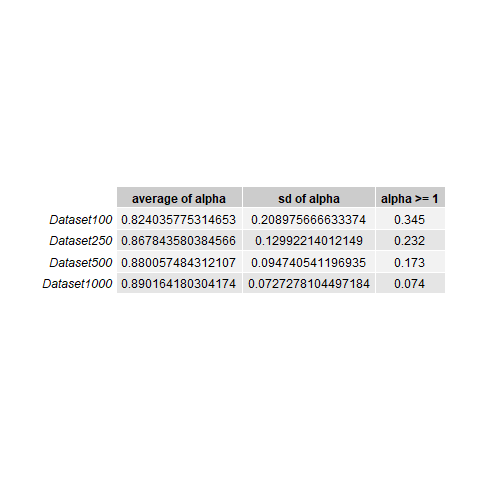
\includegraphics[scale=0.2]{C:/Users/paulina/Desktop/TeXBeamer/table 2017_12_16 205928 set seed 123 Marsenne Twister.png}
}
\frame{
\frametitle{Results with other RNG}
RNG: Knuth-TAOCP-2002
\begin{center}
\begin{tabular}{l*{6}{c}r}
n              & $k^-1\sum_{j=1}^k \hat{\alpha_j}$ & $\sqrt{k^-1\sum_{j=1}^k (\hat{\alpha_j}-\alpha)^2}$ & $ \# (\alpha_j \geq 1) $ \\
\hline
100 & 0.806 & 0.219 & 27.6\%  \\
250           & 0.852 & 0.133 &19.5\%  \\
500           &0.886 & 0.095 & 17.5\%  \\
1000     &0.893 & 0.073 & 9.2\%  \\
\end{tabular}
\end{center}

RNG: Wichmann-Hill
\begin{center}
\begin{tabular}{l*{6}{c}r}
n              & $k^-1\sum_{j=1}^k \hat{\alpha_j}$ & $\sqrt{k^-1\sum_{j=1}^k (\hat{\alpha_j}-\alpha)^2}$ & $ \# (\alpha_j \geq 1) $ \\
\hline
100 & 0.809 & 0.216 & 29.5\%  \\
250           & 0.861 & 0.134 &24.4\%  \\
500           &0.879 & 0.099 & 16.2\%  \\
1000     &0.891 & 0.073 & 9\%  \\
\end{tabular}
\end{center}
}

\frame{
\frametitle{Plots of simulated ARCH(1)}
\begin{columns}
\column{1.5in}
n=100
\includegraphics[scale=0.3]{timeSeriesDataset100.png}
\includegraphics[scale=0.3]{StandardizedResidualsDataset100.png}
\column{1.5in}
n=1000
\includegraphics[scale=0.3]{TimeSeriesDataset1000.png}
\includegraphics[scale=0.3]{StandardizedResidualsDataset1000.png}
\end{columns}
}
\frame{
\frametitle{Plots of simulated ARCH(1)}
\begin{columns}
\column{1.5in}
n=100
\includegraphics[scale=0.3]{QQplotofstandardizedresidualsDataset100.png}
\column{1.5in}
n=1000
\includegraphics[scale=0.3]{QQplotofstandardizedresidualsDataset1000.png}
\end{columns}
}


\section{Further Information}

\frame{
\frametitle{For Further Reading}
\begin{thebibliography}{aaaaaaaaaaaaaaaaa}
\beamertemplatearticlebibitems
\bibitem{Gentle:2002}
Gentle, James E.	
\newblock{\em Elements of Computational Statistics}
\beamertemplatearticlebibitems
\bibitem{Rpackage:2017}
R-Package 
\newblock{\em fGarch, Nov 2017}
\newblock available on \href{https://cran.r-project.org/web/packages/fGarch}
\beamertemplatearticlebibitems
\bibitem{Bollersev,Wooldridge:2007}
Bollersev, T. , Wooldridge, M.
\newblock{\em Quasi-maximum likelihood estimation and inference in dynamic models with time-varying covariances}
\end{thebibliography}
}
% Define the end of the document:
\end{document}
